\section{POSA}

\subsection{Whole Part}

ermöglicht Aggregation von losen zusammenhängenden Komponenten zu einer Einheit \\

\textbf{Beispiel}

\begin{itemize}
    \item Ein Auto (Whole) besteht aus vielen Parts (Räder, Schrauben, Motor usw.)
    \item 3D-Modelle bestehen aus Sub-Parts welche wiederum aus einfachen Shapes (Kreis, Dreieck etc.) bestehen
    \item Moleküle bestehen aus Atomen, welche aus Elementarteilen bestehen
    \item Stückliste einer Maschine bestehende aus Baugruppen und Bauteilen (Assemply-Parts Variante)
    \item GUI-Frameworks (Windows, Frames, Components, ...)
\end{itemize}

\subsubsection{Problem}

Fast jede Applikation basiert auf Objekten, welche wiederum auf anderen Objekten basieren. Komplexe Objekte sollten jeweils in kleinere Objekte aufgeteilt werden oder ein komplexes Objekt stellt sich zusammen aus mehreren kleineren Objekten. Dieses \textcolor{blue}{aggregierte Objekt sollte als eine Einheit angeschaut werden können (Whole)} und es gibt \textcolor{blue}{keinen direkten Zugriff auf die einzelnen Sub-Objekte} (Parts).

\subsubsection{Solution}

Besteht aus zwei Teilen, dem Whole und den darin eingekapselten Parts und ist somit sehr simple aufgebaut

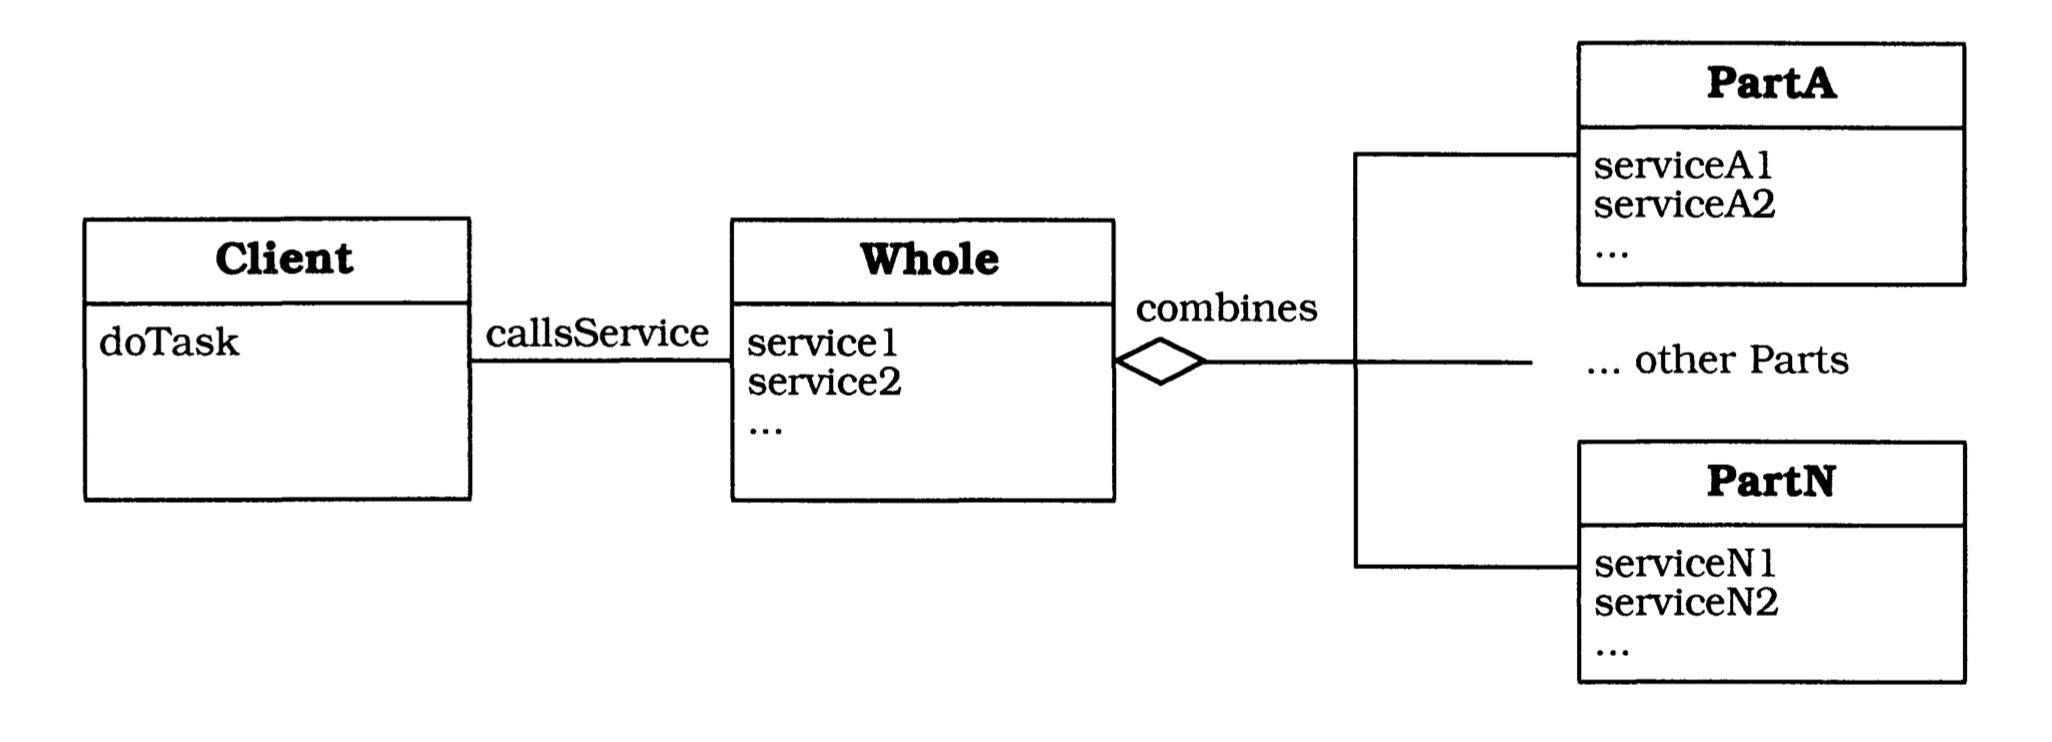
\includegraphics[width=\linewidth]{whole-part.png}

Zwei unterschiedliche Vorgehensweisen

\begin{itemize}
    \item \textcolor{blue}{bottom-up approach} vorhandene Parts in einem Whole zusammenziehen
    \item \textcolor{blue}{top-down approach} bottom-up approach Vorgehen umkehren, man erstellt die verschiedenen Parts aufgrund eines Services, welche das Whole erfüllen muss (unterteilt ein Ganzes also in kleinere Einheiten als Design-Entscheid)
\end{itemize}
\vspace{10pt}
\textbf{Varianten}, diese können auch gemischt werden.

\begin{itemize}
    \item \textcolor{blue}{Shared-Parts} der gleiche Part (Instanz) darf in verschiedenen Wholes vorkommen (shared). Dadurch ist der Lebenszyklus des Parts vom Whole losgelöst. Dies war früher ein kompliziertes Problem, da es noch keine automatischen Garbage Collectors gab. Heute ist das Aufräumen solcher Objekte nicht mehr als eigentliches Problem anzuschauen (z.B. GC in Java, Shared-Pointers in C++).
    \item \textcolor{blue}{Composite Pattern}Auf das pattern angewendbar, falls das Whole und die Parts dasselbe Interface implementieren
    \item \textcolor{blue}{Assembly-Parts} Oft kommt es vor, dass Parts wiederum Wholes bilden. So entsteht eine Baumstruktur ähnlich einer Stückliste. Beim Beispiel Auto ist das zum Beispiel der Part Reifen selbst wiederum ein ''Whole'', bestehend aus den Parts Reifen und Felgen.
\end{itemize}

\subsubsection{Einschränkungen / Zu beachten}

\begin{itemize}
    \item Parts dürfen nur in einem Whole vorkommen, da das Whole für das Instanzieren und Destruieren der Objekte verantwortlich ist (Ausnahme Variante Shared-Parts).
    \item Kein direkter Zugriff auf die Parts von aussen
    \item Das Whole darf oder soll sogar ein komplett anderes Interface wie seine Parts haben (Ausnahme Variante Composite-Pattern)
\end{itemize}

\subsubsection{Consequences}

\textbf{Vorteile}

\begin{itemize}
    \item Separation of Concerns
    \item Wiederverwendbarkeit der Parts für andere Wholes
    \item Die interne Struktur und Implementierung der Parts ist versteckt und lässt sich somit später problemlos ändern ohne das Nutzer des Wholes davon beeinflusst werden.
\end{itemize}
\vspace{10pt}
\textbf{Nachteile}

\begin{itemize}
    \item Leichter Performance-Verlust wegen der Indirection
    \item Aufteilung in die Parts kann komplex und schwierig werden
\end{itemize}

\subsection{Forwarder - Receiver}

unterstützt eine transparente Interprozess-Kommunikation (IPC). Das heisst eine Kommunikation über Systemgrenzen hinweg zwischen Peers zu ermöglichen. Die Kommunikation erfolgt über Nachrichten. \\

\textbf{Beispiele}

Im Buch vorhandene Beispiele (kennen wir alle nicht):

\begin{itemize}
    \item TASC Software Development Toolkit
    \item REBOOT Material Flow Control Software
    \item ATM-P Switching System
    \item BrouHaHA IPC in Smalltalk Environment
\end{itemize}

\subsubsection{Problem}

Um distributed applications zu ermöglichen, werden oft low-level Mechanismen für die Interprozess-Kommunikation verwendet (TCP/IP, Sockets oder Message Queues). Vorteil: Sehr effizient und fast auf allen OS vorhanden. Nachteil: Es werden Abhängigkeiten auf das verwendete OS und Netzwerk-Protokoll erstellt. Wenn ein spezifischer IPC Mechanismus verwendet wird, erschwert das die Portabilität und die Möglichkeit heterogene Umgebungen zu unterstützen.

\subsubsection{Forces}

\begin{itemize}
    \item Auswechselbarkeit der Kommunikationsmechanismen (IPC)
    \item Peer-to-Peer Model, der Sender muss nur die Namen der Empfänger kennen
    \item IPC soll nicht zu grossen Performance-Impact haben
\end{itemize}

\subsubsection{Solution}

Das Pattern beinhaltet 3 Komponenten

\textbf{Peer}

\begin{itemize}
    \item Ist für die Applikation verantwortlich resp. stellt den Service zur Verfügung
    \item \textcolor{blue}{Jeder Peer hat einen Namen} und kennt alle Namen der anderen Peers, mit denen er kommunizieren will, \textcolor{blue}{besitzt einen Forwarder und einen Receiver} für das Senden/Empfangen von Nachrichten
    \item (Jedoch auch only-way Kommunikation möglich, also entweder nur Forwarder oder nur Receiver)
\end{itemize}
\vspace{10pt}
\textbf{Forwarder}

\begin{itemize}
    \item Enthält sämtliche Funktionalität, um Nachrichten senden zu können
    \item Kann Nachrichten über Systemgrenzen hinweg senden
    \item Enthält ein Mapping zwischen den Peer-Namen und der eigentlichen physikalischen Adresse (z.B. IP).
    \item Wandelt die Nachrichten in das benötigte Format für den Transport (\textcolor{blue}{Serialisierung}, Byte-Order etc.) um und sendet diese an einen Receiver
\end{itemize}
\vspace{10pt}
\textbf{Receiver}

Enthält sämtliche Funktionalität um Nachrichten empfangen zu können

\begin{itemize}
    \item Besitzt ein Interface, um Messages zu empfangen
    \item Wandelt die empfangen Nachrichten vom Transport-Format zurück in das benötigte Format (\textcolor{blue}{Deserialisierung})
\end{itemize}

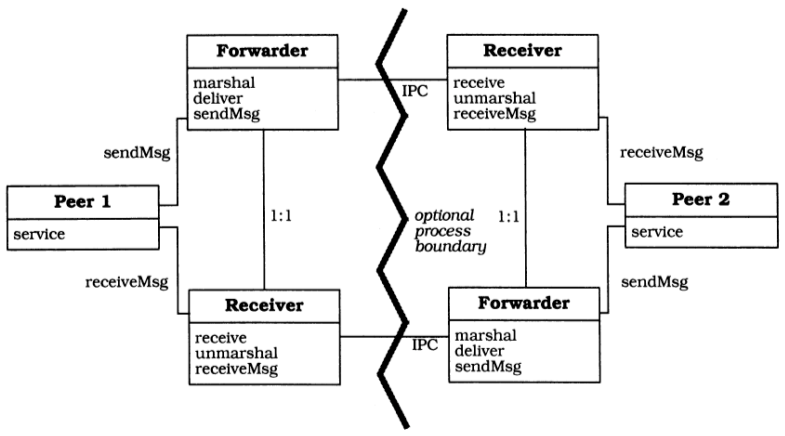
\includegraphics[width=\linewidth]{forwarder-receiver.png} \\

\textbf{Sequenzdiagramm}

Der Ablauf lässt sich sehr einfach anhand des Sequenzdiagramms verstehen

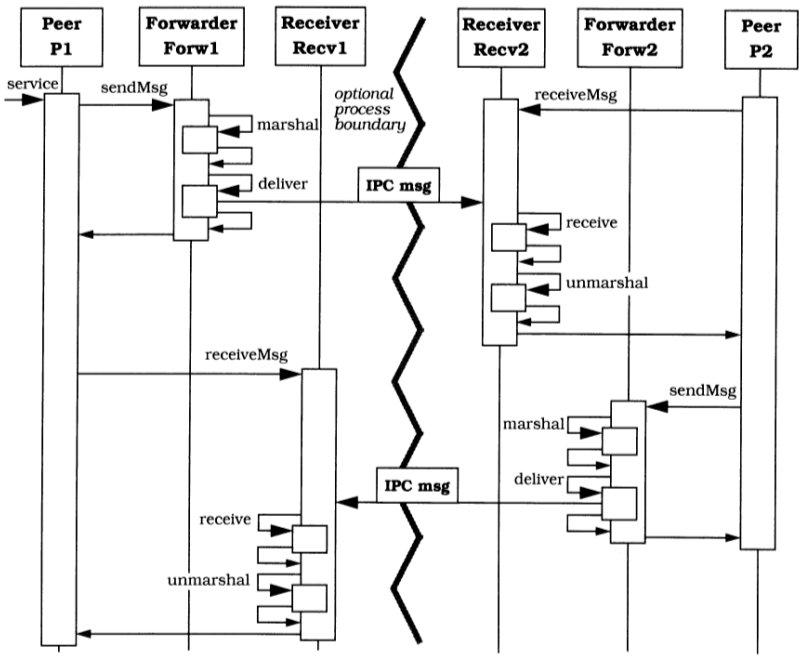
\includegraphics[width=\linewidth]{forwarder-receiver-sequencediagram.png}

\textbf{Designhinweise}

Wichtig Punkte, die beim Design beachtet werden müssen:

\begin{itemize}
    \item Ist das Empfangen von Nachrichten \textcolor{blue}{blockierend oder nicht blockierend}?
    \item \textcolor{blue}{Wie Error-Handling} bewerkstelligen?
    \item Ein gutes Naming-Systems entwickeln (z.B. Namespace/Gruppe/Name). Mehrere Peers können auch gleiche Namen oder zu Gruppen zusammengefasst werden, so ist ein hierarchisches System und Broadcasting möglich.
    \item Das System benötigt einen Startup-Mechanismus welches ein identisches Mapping Name/Adresse bei allen Peers garantiert.
    \item Der darunterliegende Kommunikationsmechanismus muss bestimmt und abstrahiert werden.
\end{itemize}
\vspace{10pt}
\textbf{Varianten}

\begin{itemize}
    \item \textcolor{blue}{Client-Dispatcher-Server} Verteilung der Komponenten ist unklar zur Compilezeit. Änderungen zur Runtime möglich, z.B. wenn ein Peer seinen Standort wechselt und eine neue physikalische Adresse erhält. Peers können sich an- und abmelden.
\end{itemize}

\subsubsection{Consequences}

\textbf{Vorteile}

\begin{itemize}
    \item \textcolor{blue}{Effiziente IPC} Kommunikation zwischen den Komponenten ist in einer Peer-to-Peer Art aufgebaut. Jeder Forwarder kennt die physikalische Adresse des potenziellen Receivers. Der Forwarder muss dadurch nicht die Receiver lokalisieren.
    \item \textcolor{blue}{Encapsulation of IPC facilities} Alle Abhängigkeiten auf konkrete IPC Implementationen werden gekapselt in Forwarder und Receiver. Eine Änderung des IPC-Mechanismus betrifft keine anderen Komponenten ausser dem Forwarder und dem Receiver.
\end{itemize}

\textbf{Nachteile}

\begin{itemize}
    \item \textcolor{blue}{Kein Support für flexible Konfiguration von Komponenten} Das Mapping zwischen Name und Adresse ist statisch, Änderungen zur Runtime sind kaum möglich. Wenn die Verteilung der Peers sich ändert, kann nicht darauf reagiert werden. Dieses Problem kann behoben werden, wenn ein zentraler Dispatcher eingesetzt wird (Client-Dispatcher-Server Pattern), wo man sich dynamisch ab- und abmelden kann.
\end{itemize}

\subsection{Blackboard}

löst Probleme ohne deterministische Lösung. Dabei arbeiten verschiedene spezialisierte Komponenten auf denselben Daten (auf dem Blackboard) um auf eine (genügend gute) Lösung zu kommen. \\

\textit{Der Name ''Blackboard'' bedeutet übersetzt so was wie Wandtafel. Es ist also eine Analogie als würden diverse Experten (Knowledge sources) gemeinsam an einer Wandtafel arbeitet. Sobald diese für sich interessante Daten auf dem Blackboard entdecken, produzieren neue Daten (Hypothesen) und schreiben sie wieder aufs Blackboard. Ein anderer Experte kann nun eventuell diese Daten wieder verwenden. Ein "Chef" (Control component) prüft derweilen, ob es schon eine genügend gute Lösung gibt und würde dann die Experten stoppen.}

\textbf{Beispiele}

\begin{itemize}
    \item \textcolor{blue}{HEARSAY-II} Spracherkennung aus den 1970er.
    \item \textcolor{blue}{HASP/SIAP} System für die Erkennung von feindlichen U-Booten mit Daten von Hydrophonen (Unterwassermic) und von händisch erfasste Geheimdienst Infos.
\end{itemize}

\subsubsection{Problem}

Transformationen von raw data nach high level data structures ist schwierig und oft nicht in einer nützlichen Zeit deterministisch lösbar. \\

Beispiel solcher Probleme: Bild-, Spracherkennung oder Überwachung. \textcolor{blue}{All diese Probleme können in verschiedene Subprobleme aufgeteilt werden.} Diese Subprobleme benötigen verschiedene spezialisierte Problemlösungsansätze. Es kann auch sein, dass die produzierten Daten mit Unsicherheiten daherkommen oder nur Annäherungen für exakte Lösungen sind. Die verschiedenen Subprobleme können auch alternative Lösungen anbieten, von denen die beste (oder die mit dem meisten Rückhalt) ausgewählt werden soll.

\subsubsection{Forces}

Bei einem Speech To Text Algorithmus würde eine Suche durch alle möglichen Lösungen zu lange dauern. Ein Satz mit zehn Wörtern mit einem Wörterbuch vom 1000 Wörter gibt es $1000^{10}$ Kombinationsmöglichkeiten.
Die Problem-Domain ist noch nicht gut erforscht und es müssen verschiedenen Algorithmen ausprobiert werden. Einzelne Module müssen schnell austauschbar sein.
Input, Intermediate und Final Resultate haben verschiedene Formate. \\

Ein Algorithmus muss auf den Resultaten eines anderen arbeiten. \\

\textcolor{blue}{AI wird als mögliche Lösung für solche Probleme angesprochen}

\subsubsection{Solution}

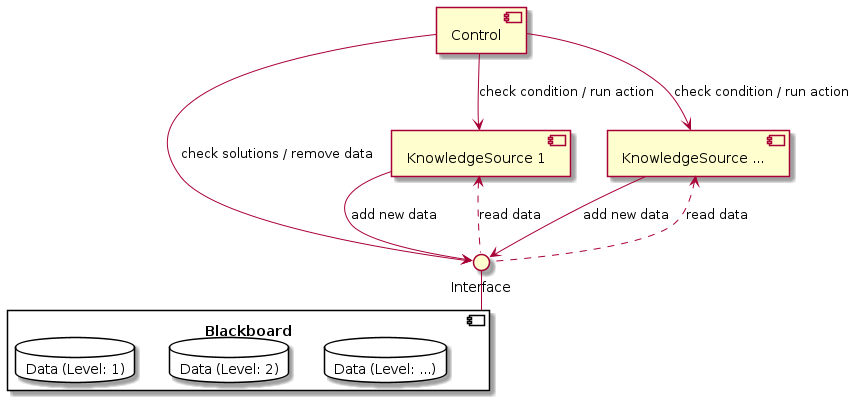
\includegraphics[width=\linewidth]{blackboard.png}

Da Blackboard-Pattern besteht aus drei Komponenten \\

\textbf{Blackboard}

Ist der \textcolor{blue}{Container für die Daten} und bietet Methoden, um auf diese zuzugreifen, neue hinzuzufügen und alte (verworfene Lösungen) zu entfernen. Ein \textcolor{blue}{Datensatz auf dem Blackboard werden auch Hypothesen genannt}. \\

Ein Datensatz hat oft mehrere Attribute, an denen eine Knowledge Source herausfinden kann, ob die Daten für ihn als Input in Frage kommt wie zum Beispiel

\begin{itemize}
    \item \textcolor{blue}{Abstractionslevel} Wie weit sind die Daten schon verarbeitet? Wie weit vom Rohzustand entfernt?
    \item \textcolor{blue}{Zeit: Wann wurde der Datensatz erstellt}
\end{itemize}
\vspace{10pt}
\textbf{Control Component}

Das Kontrollelement läuft in einer Schleife und sorgt dafür, dass falls neue Daten eine Condition einer Knowledge source erfüllen dessen Action ausgeführt wird. Es prüft ausserdem ob ungenügende Lösungen verworfen werden können und stoppt den Prozess sobald eine genügend gute Lösung gefunden worden ist. \\

\textbf{Knowledge Source(s)}

Separate und unabhängige Subsysteme die ein spezifischer Teil des Problems zu lösen versuchen. Sie transferieren ein Input von einem tieferen Abstraktionslevel auf ein höheres. Knowledge sources kommunizieren nie direkt miteinander, sondern nur mit dem Blackboard! \\

Hinweis: Knowledge sources haben zwei Methoden:

\begin{itemize}
    \item \textcolor{blue}{Eine Condition} Gibt an, ob die Komponenten den Datensatz abhängig der Attribute (Abstraktionslevel, Zeitstempel) verarbeiten kann
    \item \textcolor{blue}{Eine Action} Wenn die Condition stimmt, verarbeitet die Action den Datensatz und aktualisiert das Blackboard mit dem Output
\end{itemize}
\vspace{10pt}
\textbf{Varianten}

\begin{itemize}
    \item \textcolor{blue}{Repository} Generalisierte Variante des Blackboard-Patterns. Die Zentrale Datenstruktur wird Repository genannt. Der Unterschied zu Blackboard besteht darin, dass es keine Control-Komponente gibt. Die Repository-Architektur wird eher von User-Input oder einem externen Programm gesteuert. Als Beispiel für ein Repository kann eine Datenbank genommen werden. Diese stellt das Repository dar. Die Programme, welche darauf zugreifen sind die Knowledge Sources.
\end{itemize}

\subsubsection{Consequences}

\textbf{Vorteile}

\begin{itemize}
    \item Oft die einzige Möglichkeit für nicht-deterministische Abläufe
    \item Kann eine genügend gute Lösung für ein Problem finden, wo sonst keine Lösung gefunden werden kann (weil nicht möglich oder zu aufwändig). Das Pattern ''experimentiert'' also mit Lösungsansätzen ähnlich wie es ein Mensch tun würde
    \item Eine hohe Wartbarkeit und Auswechselbarkeit ist durch das Pattern gegeben
    \item Knowledge Sources können für andere Blackboards wiederverwendet werden
    \item Unterstützt fault tolerance und Robustheit, da es erst terminiert, wenn eine genügend gute Lösung gefunden wird.
\end{itemize}
\vspace{10pt}
\textbf{Nachteile}

\begin{itemize}
    \item Keine Garantie für eine gute Lösung / Keine Garantie das überhaupt eine Lösung gefunden wird
    \item Schwer zu testen, da es keinen deterministischen Ablauf gibt und Resultate oft nicht reproduzierbar sind
    \item Es ist schwer ein gutes Design für die Kontrollstrategie zu finden
    \item Geringe Effektivität und Overhead, da viele Lösungen produziert werden, die dann eventuell wieder verworfen werden
    \item Kein Support für Parallelität "von Haus aus" (lässt sich aber heutzutage einfach bewerkstelligen, vor allem der Zugriff auf das Blackboard muss synchronisiert werden)
\end{itemize}

\subsection{Lazy Acquisition}

Die Akquisition wird von Ressourcen auf den letzten möglichen Zeitpunkt verschoben.

\textbf{Beispiele}

\begin{itemize}
    \item \textcolor{blue}{Singleton} Das Singleton Pattern verwendet üblicherweise Lazy Instantiation.
    \item \textcolor{blue}{Haskell} Erlaubt Lazy Evaluation von Expressions. Haskell evaluiert nur so viel des Programms wie es unbedingt muss.
    \item \textcolor{blue}{JIT compilation}
\end{itemize}

\subsubsection{Problem}

Ressourcen stehen nur begrenzt zur Verfügung. Nicht ordnungsgemäss verwaltete Ressourcen können zu Engpässen im System führen und erhebliche Auswirkungen auf die Systemleistung und -stabilität haben. Um verfügbare Ressourcen sicherzustellen, wenn sie benötigt werden, beziehen die meisten Systeme die Ressourcen zur Startzeit. Die frühzeitige Beschaffung von Ressourcen führt jedoch oft zu einer Verschwendung von Ressourcen, insbesondere wenn die Ressourcen nicht sofort benötigt werden.

\subsubsection{Forces}

\begin{itemize}
    \item \textcolor{blue}{Availability} Ressourcen sollten so kontrolliert werden, dass das Risiko einer Ressourcenknappheit möglichst gering ist und immer genügend Ressourcen verfügbar sind
    \item \textcolor{blue}{Stability} Ressourcenknappheit kann die Systemstabilität beeinträchtigen und sollte deshalb ein minimaler Einfluss auf das System haben
    \item \textcolor{blue}{Quick system start-up} Das Beziehen von Ressourcen sollte so gehandhabt werden, dass es einen minimalen Einfluss auf die start-up Zeit des Systems hat.
    \item \textcolor{blue}{Transparency} Die Lösung sollte so gestaltet werden, das sie dem Nutzer gegenüber transparent ist.
\end{itemize}

\subsubsection{Solution}

\textbf{Struktur}

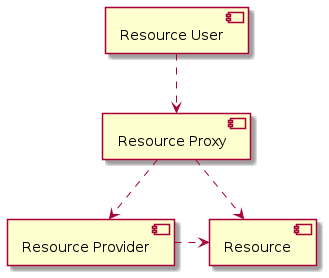
\includegraphics[width=\linewidth]{lazy-acquisition.png}

\begin{itemize}
    \item \textcolor{blue}{Resource User} Erwirbt und verwendet Ressourcen
    \item \textcolor{blue}{Resource Proxy} Fängt Akquisition der Ressourcen durch den Resource User ab und behandelt die lazily acquired Ressourcen für den Resource User
    \item \textcolor{blue}{Resource Provider} Verwaltet und stellt verschiedene Ressourcen zur Verfügung
    \item \textcolor{blue}{Resource} Entity
\end{itemize}

\textbf{Sequenzdiagramme}

\textcolor{blue}{Szenario 1}

Der Resource Provider stellt nicht nur die eigentliche Resource zur Verfügung, sondern ist gleichzeitig eine Factory für den Resource Proxy.

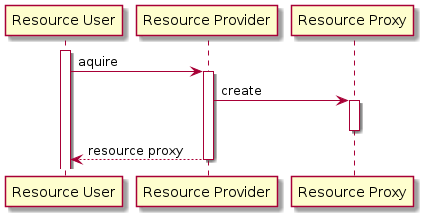
\includegraphics[width=\linewidth]{lazy-acquisition-scenario-1.png} \\

\textcolor{blue}{Szenario 2}

Der Resource User merkt nichts von der Indirektion beim Laden der eigentlichen Resource.

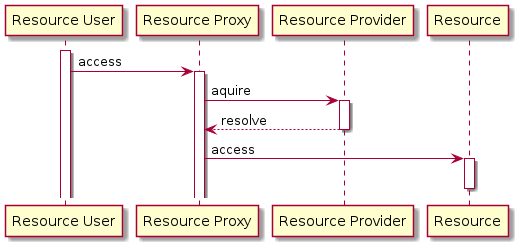
\includegraphics[width=\linewidth]{lazy-acquisition-scenario-2.png} \\

\textbf{Spezialisierungen}

\begin{itemize}
    \item \textcolor{blue}{Lazy Instantiation} Die Instanziierung eines Objektes oder einer Objektstruktur wird solange hinausgezögert bis der erste Zugriff darauf erfolgt
    \item \textcolor{blue}{Lazy Loading} Das Objekt wird erst beim ersten Zugriff geladen. Dies geschieht oft zusammen mit Lazy Instantation.
    \item \textcolor{blue}{Lazy State} Die Initialisierung des States einen Objektes erfolgt erst beim ersten Zugriff darauf. Lazy State wird häufig in Situationen verwendet, in denen nur selten auf eine grosse Menge von Zustandsinformationen zugegriffen wird. Dieses Pattern wird noch mächtiger in Kombination mit Flyweight, oder Memento.
    \item \textcolor{blue}{Lazy Evaluation} Die Berechnung des Resultates erfolgt erst, wenn auf das Resultat zugegriffen wird oder dies für eine weitere Berechnung benötigt wird. Ein Beispiel ist der \&\& Operator in vielen Sprachen. Ein weiteres Beispiel ist Haskell, dort werden Expressions erst evaluiert, wenn sie gebraucht werden (letzter möglicher Zeitpunkt).
    \item \textcolor{blue}{Lazy Initialization} Bestimmte Teile des Programms werden erst beim ersten Zugriff initialisiert. Damit wird Overhead vermieden, aber es besteht die Gefahr, dass auf nicht initialisierte Teile zugegriffen wird (NullPointerException)
    \item \textcolor{blue}{Variable Allocation} Memory wird erst dann bezogen (alloziert) wenn es benötigt wird.
\end{itemize}
\vspace{10pt}
\textbf{Varianten}

\begin{itemize}
    \item \textcolor{blue}{Semi-Lazy Acquisition} die Ressourcen werden irgendwann zwischen dem Start und dem Zugriff geladen. Dies geschieht oft im Netzwerkbereich mittels eines Netzwerk-Managers oder auch bei Betriebssystemen, die nach dem Starten weiter Module im Hintergrund laden. Ziel ist es die Vorteile von ''Laden beim Start'' und ''Beim Zugriff laden'' zu kombinieren und einen schnellen Start zu ermöglichen und die Ressource trotzdem schon bereit zu haben, wenn der Nutzer darauf zugreifen will.
\end{itemize}

\subsubsection{Consequences}

klassischer Tradeoff

\textbf{Vorteile}

\begin{itemize}
    \item \textcolor{blue}{Beim Start laden} Ressource sofort nach dem Start-up vorhanden
    \item \textcolor{blue}{Beim Zugriff laden} Schnellerer Startup
\end{itemize}
\vspace{10pt}
\textbf{Nachteile}

\begin{itemize}
    \item \textcolor{blue}{Beim Start laden} Schnellerer Startup
    \item \textcolor{blue}{Beim Zugriff laden} Der User muss beim ersten Zugriff warten
\end{itemize}

\subsection{Coordinator}

beschreibt, wie man ein System konsistent hält, indem man die verschiedenen Teilnehmer im System koordiniert. Das Pattern bietent eine Lösung für Systeme, in denen ein Task von mehreren Teilnehmern ausgeführt werden muss. \\

\textbf{Beispiele}

\begin{itemize}
    \item \textcolor{blue}{Databases} Wer das Modul DataEngeneering (DB2) gemacht hat, kennt das Two-Phase-Commit Protocol welche genau dieses Pattern anwendet.
    \item \textcolor{blue}{Software Installation} Die Installation erfolgt in zwei Schritten. Zuerst werden die Bedingungen geprüft, z.B. ob genügend Diskspace und Memory verfügbar ist und die Updateversion kompatibel ist. Erst danach wird installiert. Die ist vor allem bei Distributed Software Installationen wichtig.
\end{itemize}


\subsubsection{Problem}

In vielen Systeme müssen \textcolor{blue}{Teilnehmer den gleichen Task ausführen}. Nun kann es vorkommen, dass dieser Task bei gewissen Teilnehmern fehlschlägt, während er von anderen Teilnehmern schon erfolgreich ausgeführt wurde. Dies führt zu einem inkonsistenten System und womöglich sogar zu einem Teil- oder Totalausfall des System.

\subsubsection{Forces}

\begin{itemize}
    \item \textcolor{blue}{Consistency} Ein Task sollte entweder einen neuen Zustand im System kreieren, oder wenn er fehlschlägt den alten Zustand erhalten.
    \item \textcolor{blue}{Atomicity} Ein Task sollte entweder von allen Teilnehmern ausgeführt werden oder von keinem.
    \item \textcolor{blue}{Location tranparency} Die Lösung soll auch in distributed System funktionieren.
    \item \textcolor{blue}{Scalability} Die Lösung sollte gut skalieren, also mit mehr oder weniger Teilnehmern gut funktionieren.
    \item \textcolor{blue}{Transparency} Die Lösung soll für den User möglichst transparent sein und wenig Codeänderungen nach sich ziehen.
\end{itemize}

\subsubsection{Solution}

Es wird ein Koordinator benötig, er übernimmt die Verantwortung, dass der Task komplett ausgeführt wird. Die Participants erledigen die Arbeit, welche für den Task benötigt werden. \\

Diese Arbeit wird jeweils in zwei Teile oder Phasen geteilt

\begin{enumerate}
    \item In \textcolor{blue}{prepare} wird jeder Participant angewiesen die Aufgabe vorzubereiten. Falls der Participant dies nicht kann, so meldet er das dem Coordinator. Dieser bricht den gesamten Task ab und informiert die anderen Participants über den Abbruch (Szenario II).
    \item Bekommt der Coordinator von allen Participants ein OK, so kann er den \textcolor{blue}{commit} ausführen. In dieser Phase machen die Participants die Aufgabe wirklich. Da alle Participants sich für die Aufgabe bereit erklärt haben, wird das immer funktionieren (Szenario I).
\end{enumerate}

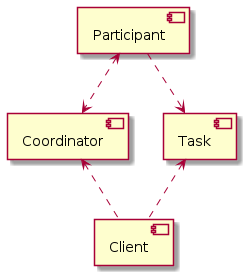
\includegraphics[width=0.5\linewidth]{coordinator.png} \\

\textbf{Participant}

Aktiver Teil, der einen Teil der Arbeit übernimmt. Er kann resource users, resource provider und resourcen beinhalten. \\

\textbf{Coordinator}

Verantwortlich für die Koordinierung so dass ein Task komplett ausgeführt wird. \\

\textbf{Task}

Unit of Work wozu mehrere Participants verwendet werden. \\

\textbf{Client}

Initiiert den Task, er sagt dem Coordinator welcher Task auszuführen ist. \\

Szenario I (success)

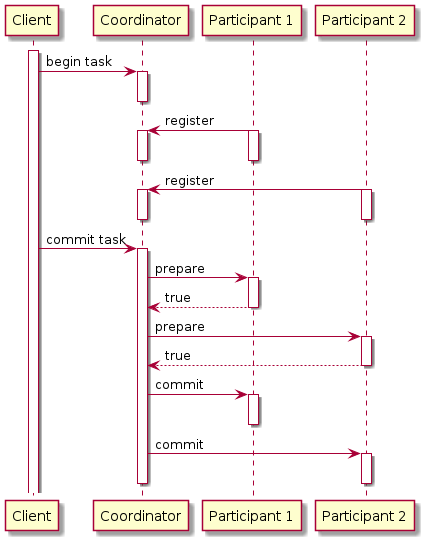
\includegraphics[width=\linewidth]{coordinator-sz-1.png} \\

Szenario II (prepare fails)

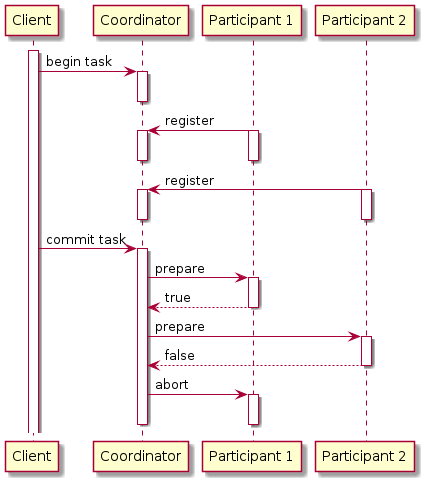
\includegraphics[width=\linewidth]{coordinator-sz-2.png}


\subsubsection{Consequences}

\textbf{Vorteile}

\begin{itemize}
    \item \textcolor{blue}{Consistency} Das System bleibt in einem konsistenten Zustand. Alle Participants haben den gleichen Stand.
    \item \textcolor{blue}{Atomicity} Ein Task wird ganz und von allen Participants oder gar nicht ausgeführt.
    \item \textcolor{blue}{Scalability} Das Pattern skaliert gut wenn Participants dazukommen
    \item \textcolor{blue}{Transparency} Die Ausführung eines Tasks ist für den Nutzer nicht sichtbar.
\end{itemize}
\vspace{10pt}
\textbf{Nachteile}

\begin{itemize}
    \item \textcolor{blue}{Overhead} Jeder Task muss in zwei Phasen aufgeteilt werden. Somit gibt es z.B. auch doppelt so viele Roundtrips im Netzwerk.
    \item \textcolor{blue}{Additional responsibility} Die Participants müssen sich beim Coorinator registrieren.
\end{itemize}

\textbf{Varianten}

\begin{itemize}
    \item \textcolor{blue}{Three-phase Commit} kann Failures in der Commit-Phase umgehen. Dazu speichert jeder Participant den Stand vor dem Commit. Schlägt bei einem Participant der Commit fehl, so meldet er es dem Coordinator welcher dann ein rollback() an alle Teilnehmer sendet, sodass diese den Vorherigen Stand wiederherstellen. Melden alle Participante ein erfolgreiches Commit, so sendet der Coordinator ein clean() was bedeutet, dass alle Commits erfolgreich waren und die Participants den gespeicherten alten Stand löschen können.
    \item \textcolor{blue}{Paricipant Adapter} Participants implementieren das Interface nicht direkt, sondern via Adapter. Hilfreich für Legacy-Code.
    \item \textcolor{blue}{Third-Party Registration} Die Participants registrieren sich nicht selbst beim Coordinator, sondern der Client übernimmt diese Aufgabe. So hat der Client die volle Kontrolle.
\end{itemize}

\subsection{Resource Lifecycle Manager (RLM)}

entkoppelt Verwaltung des Lebenszyklus von Ressourcen von ihrer Nutzung, indem ein separater Resource Lifecycle Manager eingeführt wird. Dessen einzige Aufgabe ist die Verwaltung der Ressourcen einer Applikation. \\

\textbf{Beispiele}

\begin{itemize}
    \item \textcolor{blue}{Component Container} Managed den Lifecycle einer Applikation-Komponente (J2EE, COM+)
    \item \textcolor{blue}{Remoting Middleware} Middleware Technologien wie COBRA und .NET Remoting implementieren ein RLM auf verschiedenen Levels
    \item \textcolor{blue}{Grid Computing} Dabei werden verteilte Ressourcen geteilt und aggregiert.
\end{itemize}

\subsubsection{Problem}

Das Erstellen von grossen und komplexen Systemen ist schwierig. Wenn es auch noch robust und skalierbar sein sollte, wird es noch schwieriger. Der wichtigste Punkt ist das Verwalten der Ressourcen. Das können verschiedene sein wie z.B. Netzwerkverbindungen, Threads oder Synchronisationsprimitiven. Das Verwalten solcher Ressourcen ist nicht gerade trivial. Die Ausführung eines Threads muss genau überwacht werden, um zu entscheiden, ob ein neuer erstellt werden muss oder ein alter zerstört. Dasselbe gilt für Netzwerkverbindungen, wann müssen sie verbunden oder getrennt werden? All diese Verantwortung wird durch dieses Pattern dem Resource Lifecycle Manager übergeben.

\subsubsection{Solution}

Es wird ein Resource Lifecycle Manager (RLM) eingeführt. Seine Verantwortung ist es die Ressourcen zu verwalten. Der Resource User kann Ressourcen beantragen, diese werden ggf. durch den RLM erstellt. Der RLM kennt die aktuelle Auslastung und Verwendung der Ressourcen und kann dadurch auch Anfragen eines Resource Users ablehnen (z.B. nicht genug Memory bei einer malloc Anfrage). \\

Ein RLM kann verschiedene Abstraktionsstufen repräsentieren. Er kann für nur eine oder mehrere Ressource-Typen verantwortlich sein. Wenn verschiedene Typen untereinander eine Abhängigkeit haben, so müssen die verschiedenen RLMs zusammenarbeiten. Das kann erreicht werden mit einem zentralen RLM welcher spezifische RLMs als Resource Provider verwendet oder ein RLM welcher sich nur um die Abhängigkeiten zwischen Ressourcen kümmert. In Architekturen mit vielen Layern ist auch eine Kaskade von RLM möglich.

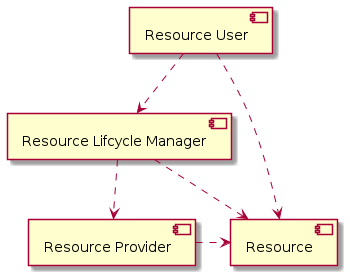
\includegraphics[width=0.5\linewidth]{resource-lifecycle-manager.png}

\textbf{Resource User}

beantragt und verwendet Ressourcen \\

\textbf{Resource Lifecycle Manager}

verwaltet den Lebenszyklus von Ressourcen, einschliesslich ihrer Erstellung/Beschaffung, Wiederverwendung und Zerstörung. \\

\textbf{Resource Provider}

besitzt und verwaltet die Ressourcen (z.B. ein OS). Der Resource Provider kann selbst ein RLM auf der gleichen oder einer anderen Abstraktionsebene sein. \\

\textbf{Resource}

eine Einheit wie eine Netzverbindung oder ein Thread \\

\textbf{Sequenzdiagramm}

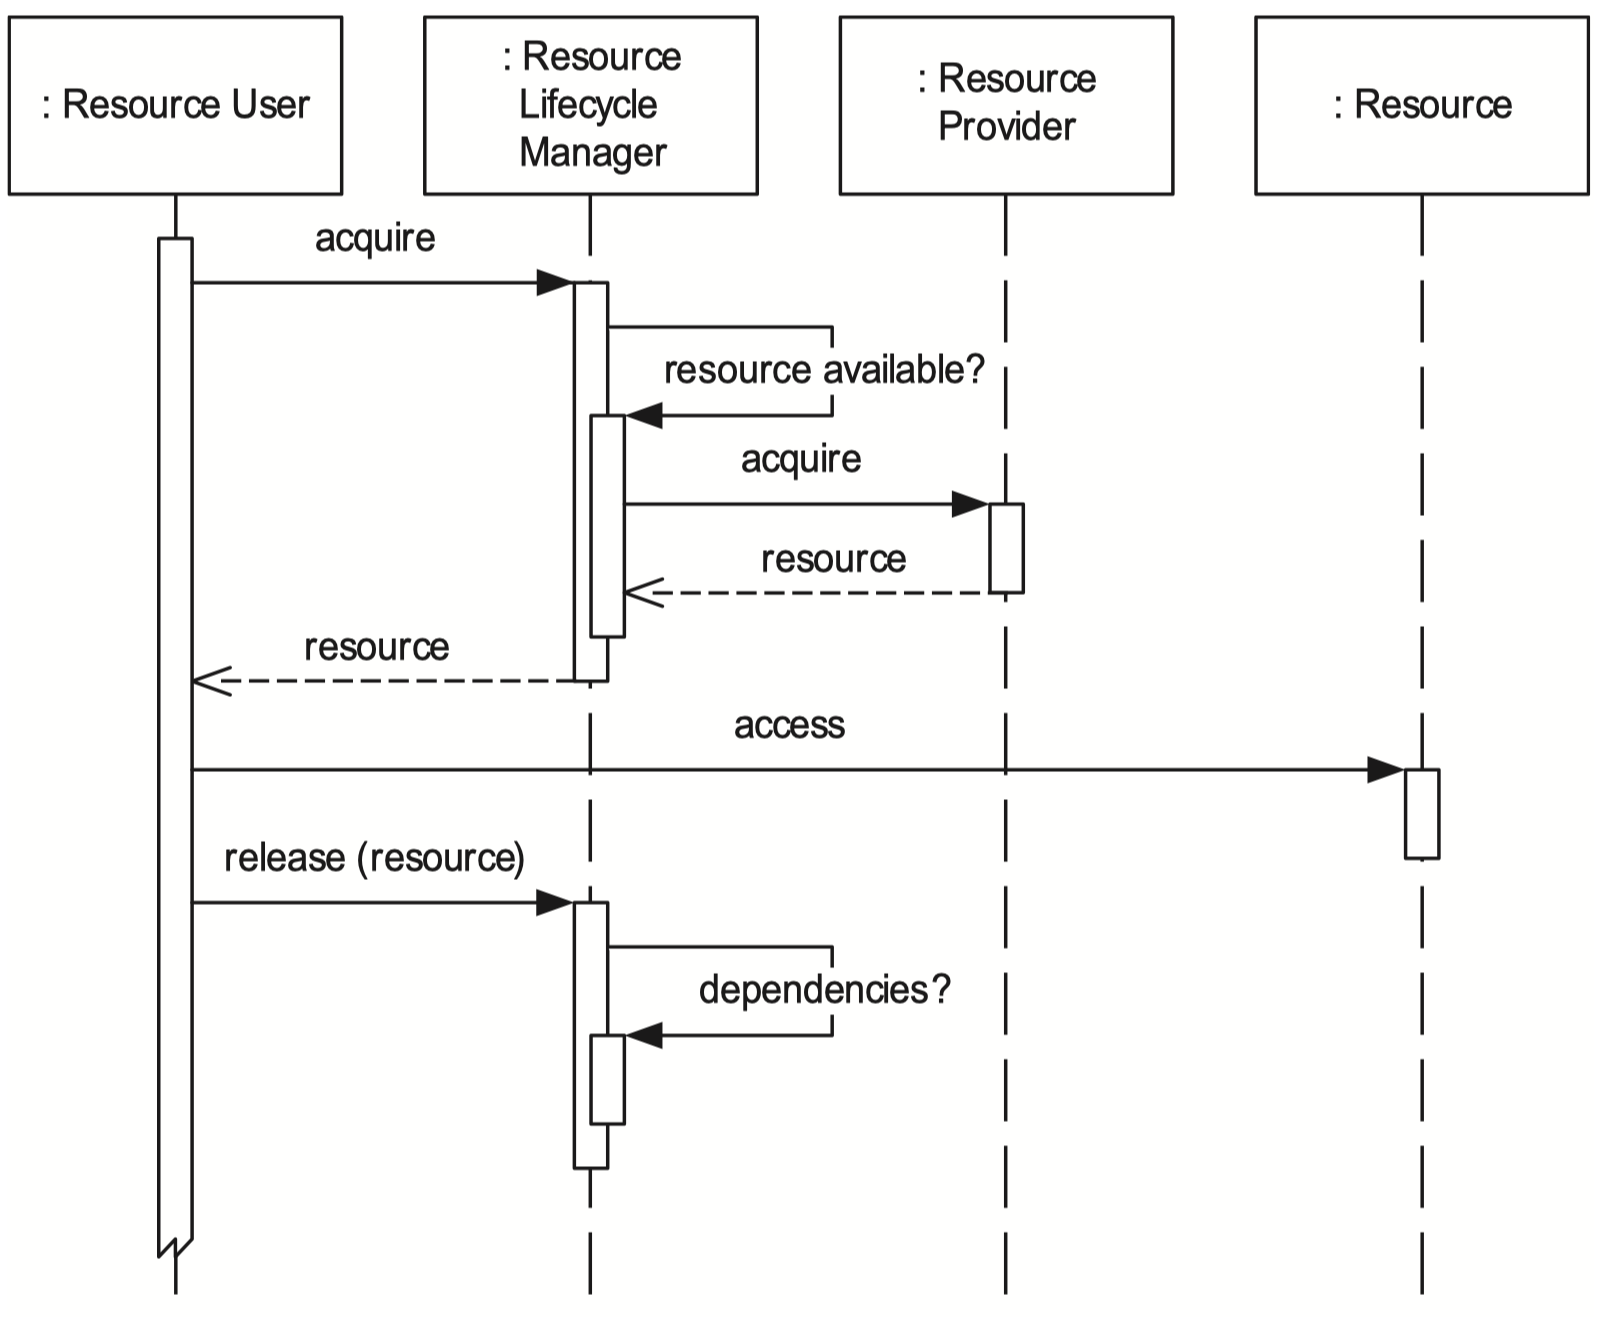
\includegraphics[width=\linewidth]{resource-lifecycle-manager-sequencediagram.png}


\subsubsection{Consequences}

\textbf{Vorteile}

\begin{itemize}
    \item \textcolor{blue}{Efficiency} Wenn jeder User seine Ressourcen selbst verwalten kann, das ineffizient sein. Diese Zentralisierung reduziert die Komplexität des Gesamtsystems
    \item \textcolor{blue}{Scalability} Das effiziente Managen der Ressourcen erlaubt die Skalierung des Systems und höhere Lasten
    \item \textcolor{blue}{Performance} Die Performance des Gesamtsystems wird erhöht
    \item \textcolor{blue}{Transparency} Die User müssen sich nicht selbst um das Managen der Ressourcen kümmern. Der Prozess ist abstrahiert und entkoppelt, sodass auch einfach Änderungen und Optimierungen möglich sind.
    \item \textcolor{blue}{Stability} Das Pattern garantiert, dass nur Ressourcen alloziert werden, wenn auch genügend Ressourcen zur Verfügung stehen. Und auch das diese wieder freigegeben werden. So wird die Stabilität erhöht. Der RLM darf auch Anfragen ablehnen, wenn nicht genügend Ressourcen zur Verfügung stehen
    \item \textcolor{blue}{Control} Mit dem Pattern hat man die volle Kontrolle über den Ressource Lifecycle. So ist es zum Beispiel auch sehr einfache einzelne Ressourcen zu tracken oder zu loggen.
\end{itemize}
\vspace{10pt}
\textbf{Nachteile}

\begin{itemize}
    \item \textcolor{blue}{Single point of failure} Ist der RLM nicht verfügbar, so ist auch das Gesamtsystem nicht verfügbar. Redundancy Konzepte helfen diesem Problem entgegenzuwirken.
    \item \textcolor{blue}{Flexibility} Wenn eine Ressource eine spezielle Behandlung benötigt, so könnte dieses Pattern eventuell zu unflexibel für das sein.
\end{itemize}


